\documentclass[border=0pt]{standalone}
\usepackage{amsmath,amssymb}
\usepackage{xcolor}
\usepackage{tikz}
\usetikzlibrary{arrows.meta,calc,decorations.pathreplacing,positioning,shapes.geometric,backgrounds}
\definecolor{c1}{RGB}{0,114,178}
\definecolor{c2}{RGB}{230,159,0}
\definecolor{c3}{RGB}{0,158,115}
\definecolor{cr}{RGB}{213,94,0}
\tikzset{every picture/.append style={show background rectangle,
    background rectangle/.style={fill=white}, inner frame sep=8pt}}
\newcommand{\roll}{\mathcal{R}}
\begin{document}
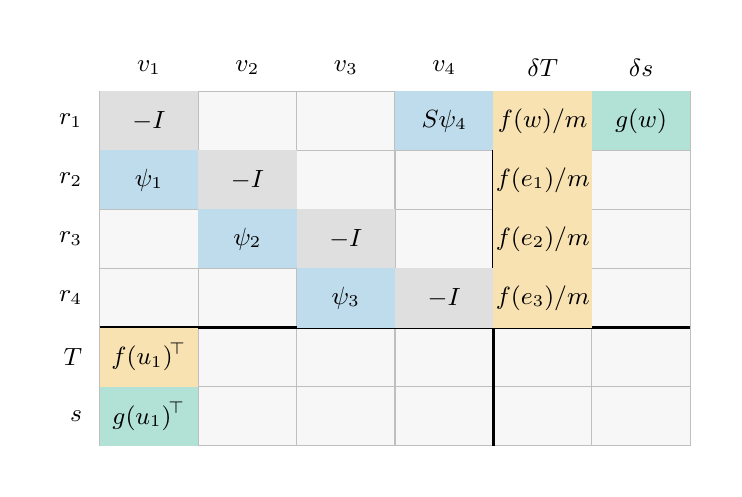
\begin{tikzpicture}[cell/.style={minimum width=1.25cm, minimum height=0.75cm, inner sep=0pt,
      font=\small}]
    \def\w{1.25}
    \def\h{0.75}
    % frame and grid
    \fill[gray!6] (0, 0) rectangle (6*\w, -6*\h);
    \draw[gray!50] (0, 0) grid[xstep=\w, ystep=\h] (6*\w, -6*\h);
    \draw[thick] (4*\w, 0) -- (4*\w, -6*\h);
    \draw[thick] (0, -4*\h) -- (6*\w, -4*\h);
    % blocks
    \newcommand{\blk}[4]{\fill[#4] ({(#2-1)*\w}, {-(#1-1)*\h}) rectangle ({#2*\w}, {-#1*\h});
      \node[cell] at ({(#2-0.5)*\w}, {-(#1-0.5)*\h}) {#3};}
    \blk{1}{1}{$-I$}{gray!25}
    \blk{2}{2}{$-I$}{gray!25}
    \blk{3}{3}{$-I$}{gray!25}
    \blk{4}{4}{$-I$}{gray!25}
    \blk{2}{1}{$\psi_1$}{c1!25}
    \blk{3}{2}{$\psi_2$}{c1!25}
    \blk{4}{3}{$\psi_3$}{c1!25}
    \blk{1}{4}{$S\psi_4$}{c1!25}
    \blk{1}{5}{$f(w)/m$}{c2!30}
    \blk{2}{5}{$f(e_1)/m$}{c2!30}
    \blk{3}{5}{$f(e_2)/m$}{c2!30}
    \blk{4}{5}{$f(e_3)/m$}{c2!30}
    \blk{1}{6}{$g(w)$}{c3!30}
    \blk{5}{1}{$f(u_1)^{\!\top}$}{c2!30}
    \blk{6}{1}{$g(u_1)^{\!\top}$}{c3!30}
    % labels
    \foreach \j/\l in {1/v_1, 2/v_2, 3/v_3, 4/v_4, 5/\delta T, 6/\delta s} {
      \node[font=\small] at ({(\j-0.5)*\w}, 0.3) {$\l$};
    }
    \foreach \i/\l in {1/r_1, 2/r_2, 3/r_3, 4/r_4, 5/T, 6/s} {
      \node[font=\small, anchor=east] at (-0.1, {-(\i-0.5)*\h}) {$\l$};
    }
  \end{tikzpicture}
\end{document}
